% Input from Bo and Lee Greenler on the TPC detail design

\subsubsection{Anode Plane Assemblies (APAs)}

% input from Lee Greenler



\begin{figure}[!htb]
\centering
\begin{minipage}[b]{1.0\textwidth}
\begin{center}
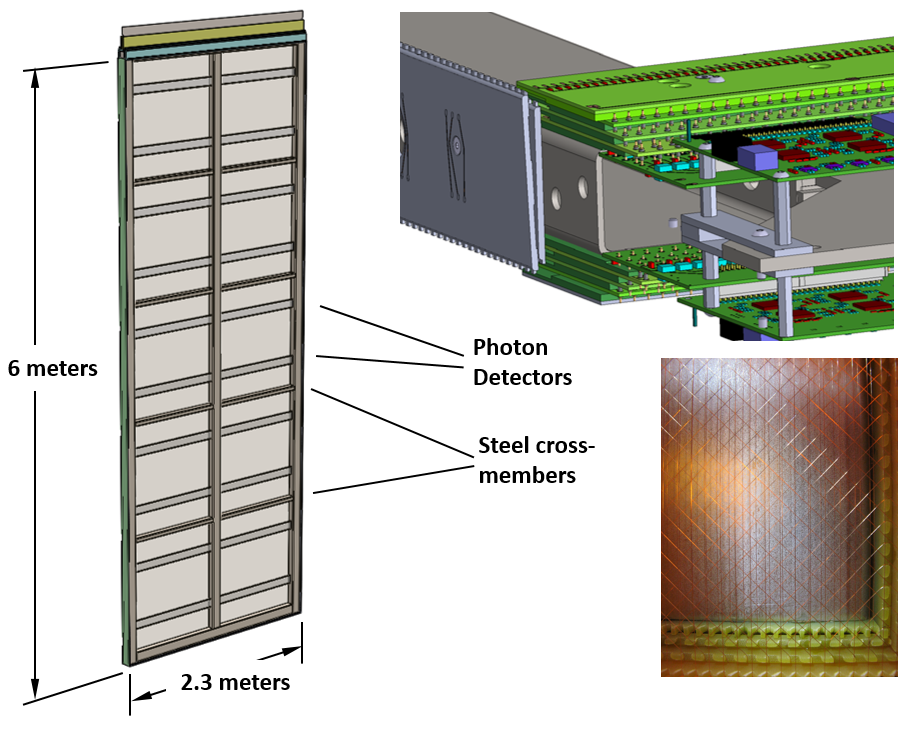
\includegraphics[width=.75\textwidth]{./figures/TPC_APA_1}
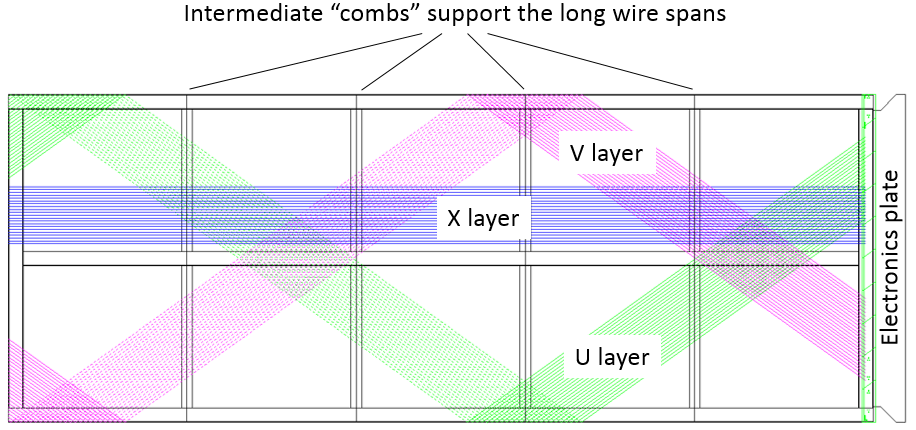
\includegraphics[width=0.75\textwidth]{./figures/TPC_APA_2}
\end{center}
\end{minipage}
\caption{Clockwise from left: A full size APA, an APA corner showing the electronics boards, an APA lower corner photo showing wires and edge boards, and a figure showing the wire orientations and the placement of wire aligning combs. }
\label{fig:tpc_apa_overview} 
\end{figure}


Each APA (Figure \ref{fig:tpc_apa_overview}) is instrumented with 3 layers of signal wires, one longitudinal collection plane and two 35.7$^\circ$ angled induction planes with an additional outer grid plane that helps maintain the field. The overall dimensions of the active area as mentioned able are 2.3 m wide, 6 m long. The dimension of the wire planes were selected to fit down the Ross shaft at SURF, be compatible with a standard HiCube transport container, and allow construction from readily available materials.  The angled layers start at the electronics end and wind around to the other side on their way to the bottom. The wire angle was selected so that a given angled induction wire will not overlay any longitudinal collection wire more than once in order to reduce ambiguities caused by the wrapped wire construction. Partial wire layers are shown here in Figure ~\ref{fig:tpc_apa_overview} at the bottom.  With a wire pitches of 4.67 mm (diagonal layers) and 4.79 (straight layers), the total number of readout channels in an APA is 2560.
The grid layer is not depicted in Figure ~\ref{fig:tpc_apa_overview} for clarity. The underlying structure of each APA is a framework of rectangular, stainless steel tubing.  The side and bottom edges of the frame are lined with multiple layers of fiberglass circuit boards, notched along the edges to support and locate the wires that cross the APA face. A set of FR4 combs are glued to the APA frame to capture the wires at regular intervals. The front-end electronics boards are mounted at the top end of the frame and protected by a metal enclosure. 


The distance between wire planes is 4.8 mm (3/16 in) corresponding with standard printed circuit board thickness, and while maintaining optimal signal formation. The four wire planes will be electrically biased so that electrons from an ionizing-particle track completely drift past the first three planes and are collected by the fourth plane. Calculations show that the minimum bias voltages needed to achieve this goal are $V_G$ = -665V, $V_U$ = -370V, $V_V$ = 0V and $V_X$ = 820V respectively (where G, U, V, and X are the wire-layer labels from outside in, towards the frame).  It is convenient to set one of the wire planes to ground so that the wires can be DC coupled to the front-end readout electronics. In this instance, the V wire plane is set to ground potential to reduce the maximum bias voltages on the other wire planes, and enable the use of lower voltage rated AC coupling capacitors. A grounded mesh plane, located 4.8 mm behind the collection (X) plane, prevents the electric field around this set of wires from being distorted by the metal frame structure and the wires on the opposite side of the frame. It also shields the sensing wires from potential EM interferences from the photon detectors (Fig.~\ref{fig:pd_insertion}) mounted within the frame. The mesh should have a wire pitch less than 2 mm to ensure a uniform electric field while maintaining a high optical transparency.


\begin{figure}[t]
  \centering
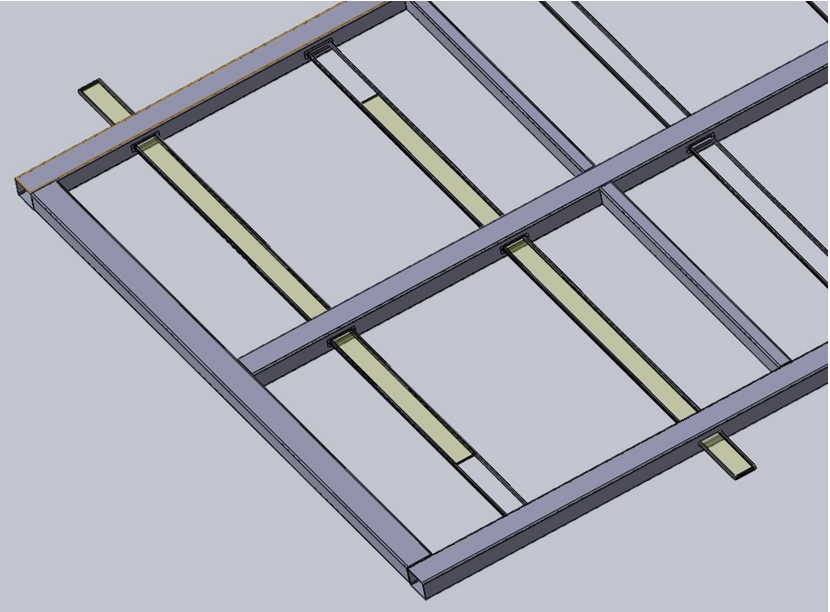
\includegraphics[width=4in]{figures/TPC_APA_3}
\label{fig:pd_insertion}
  \caption{Photon detectors are mounted within the frame, between the wires on the two sets of four wire layers.  The APA is built so that the photon detectors can be installed through slots in the side of the APA after the APA wires are installed.  The wires that would cross these slots are routed around using copper traces on the edge boards.}
\end{figure}


\subsubsection{CPA and Field Cage}

% input from Bo Yu


Each cathode plane (Fig.~\ref{fig:tpc_cpa_1}) is constructed from 6 identical CPA (cathode plane assembly) modules and two sets of end pieces. Each CPA is about half the size of an APA  (2.3m $\times$ 3.1m) for ease of assembly and transport.  The CPA is made of a stainless-steel framework, 
with 4 pieces of thin FR4 sheets mounted in the openings.  A receptacle for the HV feedthrough is attached to the upper corner of a cathode plane toward the roof entrance side to mate with the HV feedthrough in the cryostat ceiling. 

The FR4 sheets on the CPAs are treated with layers of high resistive coating on both sides.  The resistivity of the coating will be chosen such that the surface potential does not deviate significantly with the ionization current from the cosmic rays, and forms a relatively long time constant to dissipate the stored energy on each sheet in case of a high voltage discharge.  This long RC time constant will also reduce the peak current injected into the front-end electronics in a HV discharge.

Due to the relatively high cosmic ray flux in this surface detector, it is preferable to prevent the scintillation light emitted by a cosmic ray between the cathode and cryostat wall from entering the TPC to reduce false trigger. The opaque cathode surface will service this purpose. The high flux of cosmic rays combined with very low drift velocity of positive ions in the liquid argon will result in sizable space charge distortions in the TPC (docdb \#6471).  In addition, the positive ions could build up further if the ion motion is slowed or stalled by counter flow in the LAr.  Preliminary CFD analysis (docdb \#6140) have shown that solid cathodes in the cryostat result in LAr flow pattern that neither causes excess positive ion buildup, nor degrades the LAr purity.


\begin{figure}[t]
\centering
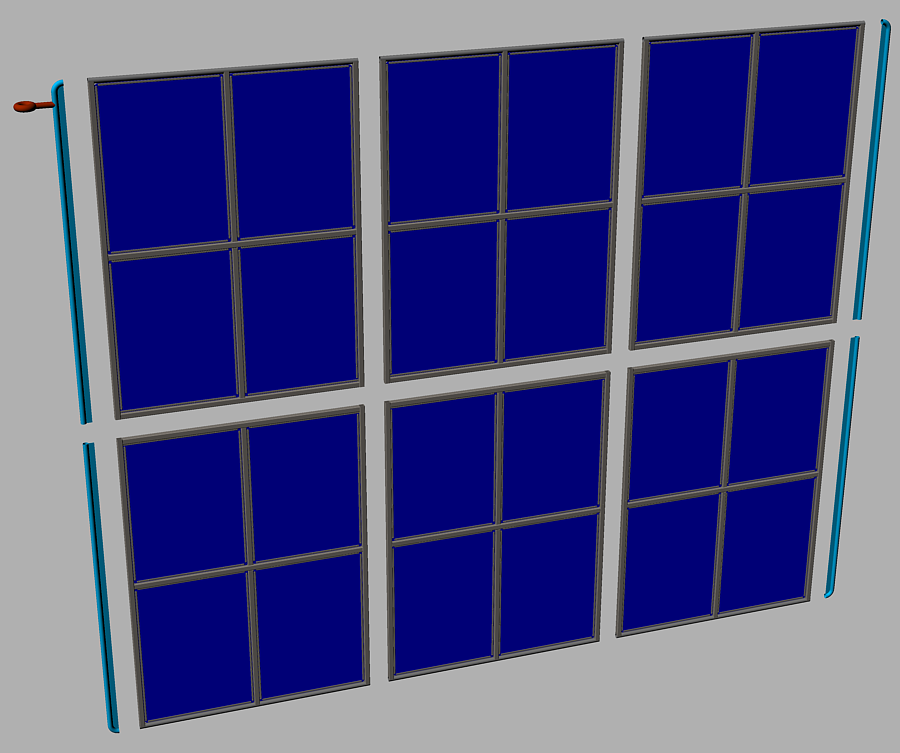
\includegraphics[width=5in]{figures/TPC_CPA_1}
\caption{Exploded view of a cathode plane constructed from 6 CPA modules and 4 end pieces. The facing material on the CPA is highly resistive to minimize the peak energy transfer in case of a HV breakdown.}
\label{fig:tpc_cpa_1}
\end{figure}

To achieve a 500~V/cm drift field over a 2.5~m distance, the bias 
voltage on the cathode plane must reach $-$125~kV. Two high voltage power supplies (150 -- 200 kV) and two HV feedthroughs will be needed for the two cathode planes.  The HV feedthroughs are based on the Icarus design, but modified to further improve the stability at higher voltages. %(Fig.~\ref{fig:tpc_hv_ft}).

%\begin{figure}[hb]
%\centering
%\includegraphics[width=5in]{figures/TPC_HV_FT}  (`figure not found' -- add it then uncomment)
%\caption{Cross section of the HV feedthrough around the end of the grounded shield, and plot of the equi-potential contours between the HV central conductor and the ground shield. The flared end significantly reduces the electric field at the inside of the shield, improving HV stability.}
%\label{fig:tpc_hv_ft}
%\end{figure}



Each pair of facing cathode and anode rows forms an electron-drift region.  A field cage  completely surrounds the four open sides of this region to provide the necessary boundary conditions to ensure a uniform electric field within, unaffected by the presence of the cryostat walls.

\begin{figure}[htb]
\centering
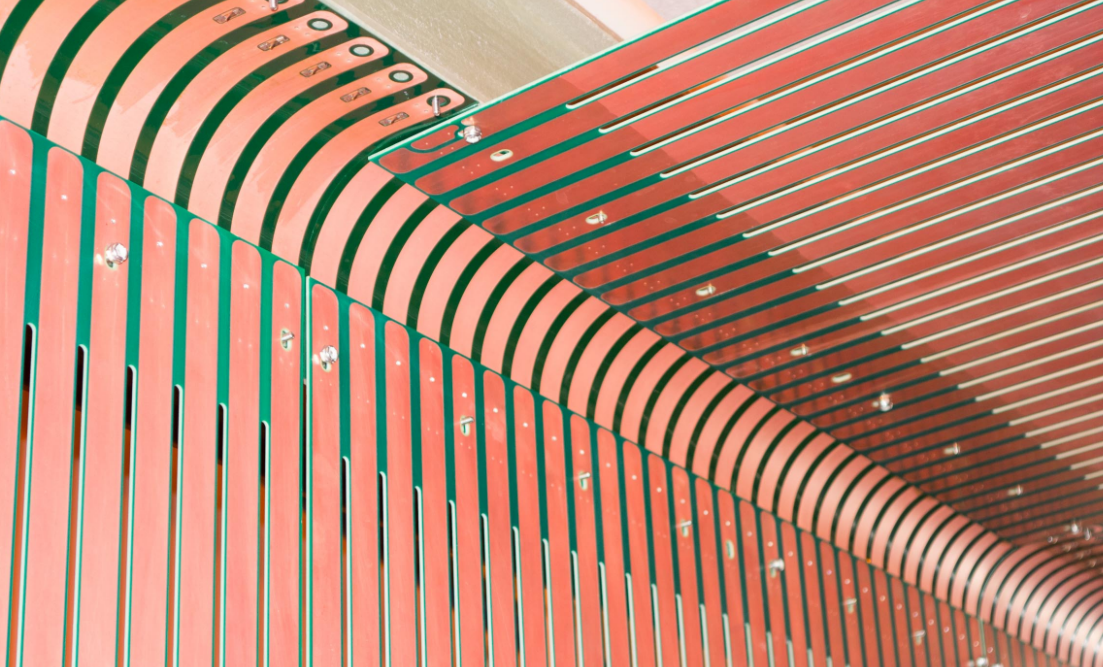
\includegraphics[width=.49\textwidth]{figures/TPC_FCA_1}
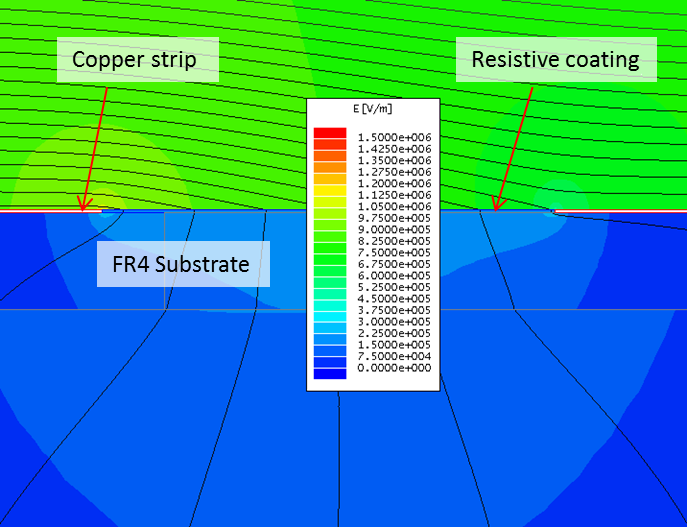
\includegraphics[width=.49\textwidth]{figures/TPC_FCA_2}
\caption{Left: A section of the field cage in the 35ton TPC. Right: Plot of electric field (color contours( and equi-potential contours (black lines) in a small region around the edges of two adjacent field cage strips on a 1.6mm thick FR4 substrate.  A layer of resistive coating between the two copper strips nearly eliminated the high electric field regions at the copper edges }
\label{fig:tpc_fca_1}
\end{figure}    

   

The field cages are constructed using copper-clad FR4 sheets reinforced with fiber glass I-beams to form panels of 2.5~m $\times$ 2.3~m in size for the top and bottom modules, and 2.5~m $\times$ 2~m modules for the sides.  Parallel copper strips are etched or machined on the FR4 sheets.  Strips are biased at appropriate voltages through a resistive divider network. These strips will create a linear electric-potential gradient in the LAr, ensuring a uniform drift field in the TPC's active volume. 
 
Since the field cage completely encloses the TPC drift region on four (of six) sides, with the remaining two sides blocked by the solid cathodes, the FR4 sheets must  be frequently perforated to allow natural convection of the liquid argon.  The ``transparency'' of the perforation will be determined by a detailed LAr computerized fluid dynamic (CFD) study.

The left of Figure~\ref{fig:tpc_fca_1} shows a section of the field cage in the 35ton TPC as it was being assembled.  The 35ton TPC test results will inform us whether we should improve upon the current design, or change the design concept all together for this and future detectors.  The main concern with the current field cage design is that the electric field at the edges of the copper strips is still quite high due to the thinness of the copper.  One possible remedy is to cover the entire surface of the field cage with a high resistive coating.  The resistivity between strips due to this coating must be kept many orders of magnitudes higher than the divider resistance to avoid distortion to the drift field.  Figure~\ref{fig:tpc_fca_1} (Right-Panel) shows an FEA simulation of such a configuration.

In the event of HV discharge on the cathode or the field cage, the voltage differential between neighboring field cage strips near the discharge electrode will be very high for a brief moment.  This over voltage condition could cause damage to the field cage electrode and the resistors installed between strips.  To minimize such disk, varistors or gas discharge tubes (GDT) will be installed between the field cage strips in parallel with the resistors to prevent excess voltage transient between the electrodes. 

In order to test the installation concept of the far detector, the top and bottom field cage modules will be attached to the mating CPAs through hinges.  These combined assembly will be installed into the cryostat and the field cage module opens to bridge the CPA and the APA both mechanically and electrically. 






